\documentclass[tikz, border=10pt]{standalone}

\usepackage{tikz}
\usetikzlibrary{mindmap, shadows}

\tikzstyle{every node} = [font=\footnotesize\sffamily\bfseries, circular drop shadow]

\begin{document}
    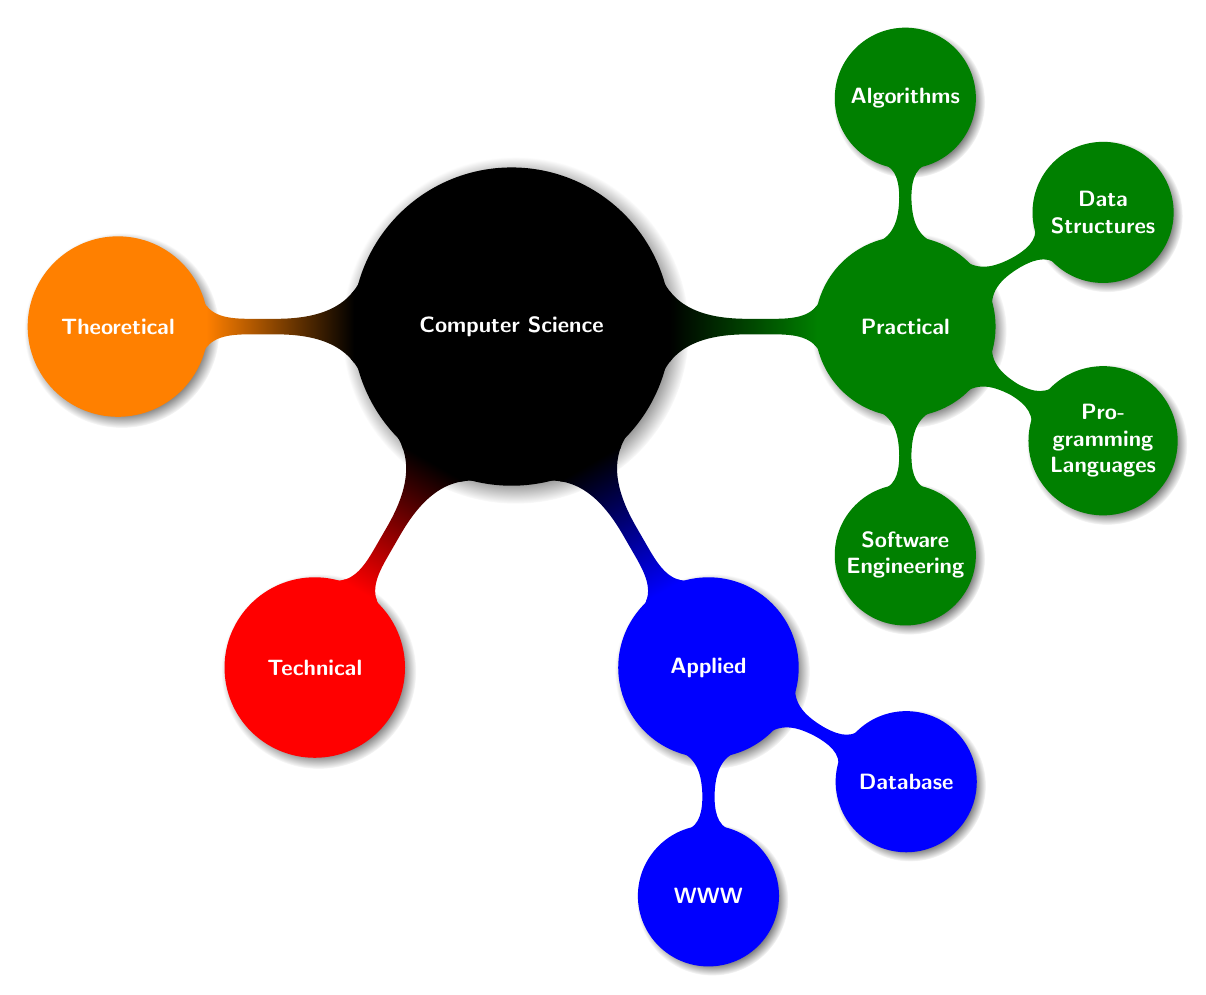
\begin{tikzpicture}
        \path[mindmap, concept color=black, text=white]
            node[concept]{Computer Science}
            [clockwise from=0]
                child[concept color=green!50!black] {
                    node[concept] {Practical}
                    [clockwise from=90]
                    child {node[concept] {Algorithms}}
                    child {node[concept] {Data Structures}}
                    child {node[concept] {Pro\-gramming Languages}}
                    child {node[concept] {Software Engineer\-ing}}
                }
                child[concept color=blue] {
                    node[concept] {Applied}
                    [clockwise from=-30]
                    child {node[concept] {Database}}
                    child {node[concept] {WWW}}
                }
                child[concept color=red] {
                    node[concept] {Technical}
                }
                child[concept color=orange] {
                    node[concept] {Theoretical}
                };
    \end{tikzpicture}
\end{document}